% % Let 
% % \begin{align}
% %     \vec{A} = \myvec{-5\\12}, \vec{B{} = \myvec{9\\-2}$
% % \end{align}
% % Then 
% % \begin{align}
% %     \vec{C}&=\frac{{B}+{A}}{1+1}=\frac{{B}+{A}}{2}\\
% %     &= \frac{\myvec{9\\-2}+\myvec{-5\\12}}{2}\\
% %     \implies {C}&= \myvec{2\\5}
% % \end{align}
% % And now we have to find the ratio in which C divides the line
% % joining the points P = $\myvec{-8\\-5}$ and Q = $\myvec{7\\10}$. Let the ratio is $k:1$,
% % Then,
% % \begin{align}
% %     \implies {C}&=\frac{k{Q}+{P}}{k+1}\\
% %     \myvec{2\\5} &= \frac{{k{\myvec{7\\10}+\myvec{-8\\-5}}}}{k+1}\\
% %     \myvec{2\\5}&=\frac{1}{k+1} \myvec{7k-8\\10k-5}\\
% %     \implies k &= 2
% % \end{align}
% % As $k=2$, That implies C divides the line
% % joining the points P = $\myvec{-8\\-5}$ and Q = $\myvec{7\\10}$ in the ratio $2:1$.

% % $\therefore$ C is point of trisection of line joining P and Q.

% \begin{figure}[htp]
%     \centering
%     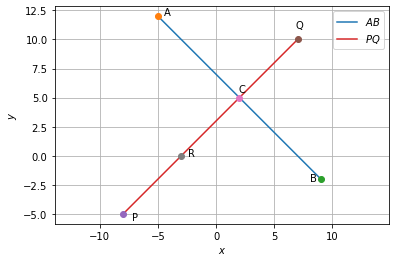
\includegraphics[width=\columnwidth]{solutions/1/1/14/a_1.png}
%     \caption{}
%     \label{fig:ramsey/1/1/14/}
% \end{figure}

% $\therefore$ The middle point of the line joining the points $\myvec{-5\\12}$ and $\myvec{9\\-2}$ is a point of trisection of the line
% joining the points $\myvec{-8\\-5}$ and $\myvec{7\\10}$.

